\chapter{Q-Learning}




\section{Reinforcement Learning}

Reinforcement learning (RL) refers to both a learning problem and a subfield of machine
learning. As a learning problem, it refers to learning to control a system so as to maximize
some numerical value which represents a long-term objective. A typical setting where
reinforcement learning operates is shown in Figure 1: A controller receives the controlled
system’s state and a reward associated with the last state transition. It then calculates an
action which is sent back to the system.


\begin{figure}
\centering
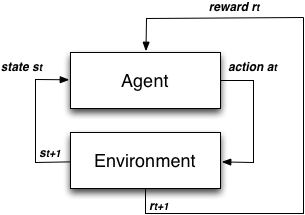
\includegraphics[width=0.7\textwidth]{./images/agentenv.png}
\caption{Example of a simple MDP with three states and two actions}
\label{fig:agentenv}
\end{figure}


The basis idea of Reinforcement learning  is simply to capture the most important aspects of the real problem facing a learning agent interacting with its environment to achieve a goal \cite{Sutton2012}. Reinforcement learning is learning what to do—how to map situations to actions—so as to maximize a numerical reward signal. The learner need to discover which actions yield the most reward by trying them \cite{Sutton2012}.

In Reinforcement Learning, an agent wanders in an unknown environment and tries to maximize its long term return by performing actions and receiving rewards. The challenge is to understand how a current action will affect future rewards. A good way to model this task is with Markov Decision Processes (MDP), which have become the dominant approach in Reinforcement Learning.

In Reinforcement Learging, all agents act in two phases: Exploration vs Explotation. In Exploration phase, the agents tries discover better action selections to improve its knowledge. In Explotation phase, the agents tries to maximize its reward, based on what its already know.

One of the challenges that arise in reinforcement learning is the trade-off between exploration and exploitation. To obtain a lot of reward, a reinforcement learning
agent must prefer actions that it has tried in the past and found to be effective in producing reward.
But to discover such actions, it has to try actions that it has not selected before. The agent has to exploit what it already knows in order to obtain reward, but it also has to explore in order to make better action selections in the future.


\subsection{Markov decision processes}

Markov decision processes (MDPs) provide a mathematical framework for modeling decision making. A countable MDP is defined as a triplet $M=(\chi,A,P_{0})$ \cite{Szepesvari2010}. where $\chi$ is a set of states, A is a set of actions. The transition probability kernel $P_{0}$ assigns to each state-action pair $(x, a) \in \chi x A $


The six main elements of a MDP are:(1) state of the system, (2) actions, (3) transition probabilities, (4) transition rewards, (5) a policy, and (6) a performance metric \cite{Sutton2012}.

\begin{figure}
\centering
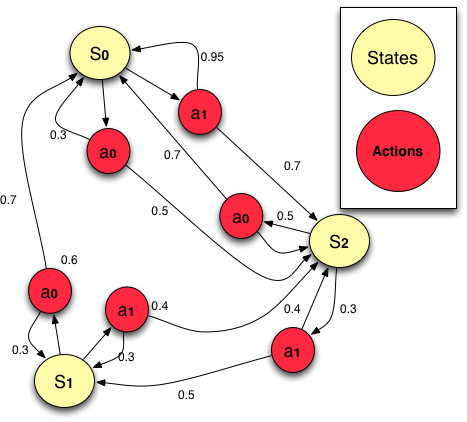
\includegraphics[width=0.7\textwidth]{./images/mdp1.png}
\caption{Example of a simple MDP with three states and two actions}
\label{fig:mdp}
\end{figure}


The state of a system is a parameter or a set of parameters that can be used to describe a system. For example the geographical coordinates of a robot can be used to
describe its state. A system whose state changes with time is called a dynamic system. Then it is not hard to see why a moving robot produces a dynamic system.

Actions are the controls allowed for an agent. Transition Probability denotes the probability of going from state i to state j under the influence of action a in one step. If an MDP has 3 states and 2 actions, there are 9 transition probabilities per action. Usually, the system receives an immediate reward ,which could be positive or negative, when it transitions from one state to another

A policy defines the learning agent’s way of behaving at a given time. Roughly speaking, a policy is a mapping from perceived states of the environment
to actions to be taken when in those states. It corresponds to what in
psychology would be called a set of stimulus–response rules or associations.  Policys mapping from states to actions.

Performance Metric: Associated with any given policy, there exists a so-called performance
metric — with which the performance of the policy is judged. Our goal is to select the policy
that has the best performance metric. 

\subsection{Types of Control Learnings}


Fig. shows the basic types of control learning problems. The first criterion that the space of problems is split upon is whether the learner can actively influence the observations.In case she can, then we talk about interactive learning, otherwise one is facing a non-interactive learning problem.

Interactive learning is potentially easier since the learner has the additional option to influence the distribution of the sample. However, the goal of
learning is usually different in the two cases, making these problems incomparable in general.

In the case of non-interactive learning, the natural goal is to find a good policy given the observations.
A common situation is when the sample is fixed. For example, the sample can be the result of some experimentation with some physical system that happened before learning started. 

Consider now interactive learning. One possibility is that learning happens while interacting
with a real system in a closed-loop fashion. A reasonable goal then is to optimize online performance,
making the learning problem an instance of online learning. Online performance
can be measured in different ways. A natural measure is to use the sum of rewards incurred
during learning. 




\section{Q-Learning}

Q-learning is a model-free reinforcement learning technique. Q-learning, it is a multiagent learning algorithm that learns equilibrium policies in Markov games, just as Q-learning learns to optimal policies in Markov decision processes \cite{Greenwald2003}. 

Q-learning and related algorithms tries to learn the optimal policy from its history of interaction with the environment. A history of an agent is a sequence of state-action-rewards.Where $s_{n}$ it is a state, $a_{n}$ it is an action and $r_{n}$ is a reward:

\begin{equation}
<s_{0},a_{0},r_{1},s_{1},a_{1},r_{2},s_{2},a_{2},r_{3},s_{3},a_{3},r_{4},s_{4}....>,
\end{equation}


In Q-Learning, the system's objective is to learn a control policy $\pi = \sum_{n=0}^{\infty} \gamma\textsuperscript{n}  r_{t}+n $, where $\pi$  is the discounted cumulative reward, $\gamma$ is the discount rate ($01$) and $r_{t}$ is the reward reiceved after execution an action at time t.

\section{GridWorld Example}

The GridWorld problem is an example of using reinforcement learning with Q-Learning. In this example extracted from \url{http://www.cs.ubc.ca/~poole/demos/rl/q.html}, there are four rewarding states (apart from the walls), one worth +10 (at position (9,8); 9 across and 8 down), one worth +3 (at position (8,3)), one worth -5 (at position (4,5)) and one -10 (at position (4,8)). In each if these states the agent gets the reward when it carries out an action in that state.

The numbers in the squares shows the Q-values of the square for each action. The blue arrows show the optimal action based on the current value function.

\begin{figure}
\centering
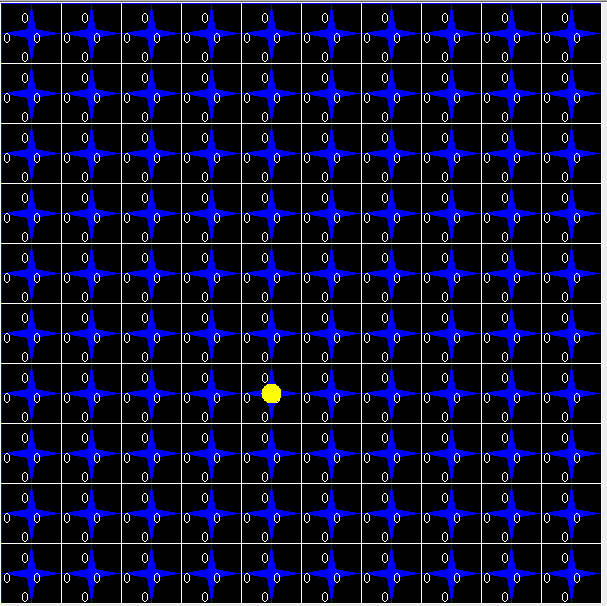
\includegraphics[width=0.7\textwidth]{./images/grid1.png}
\caption{Example of a simple MDP with three states and two actions}
\label{fig:mdp}
\end{figure}



There are 4 actions available: up, down, left and right. If it carries out one of these actions, it have a 0.7 chance of going one step in the desired direction and a 0.1 change in going one step in any of the other three directions. If it bumps into the outside wall (i.e., the square computed as above is outside the grid), there is a penalty on 1 (i.e., a reward of -1) and the agent doesn't actually move. When an agent acts in one of the states with positive reward, it is flung, at random, to one of the 4 corners of the grid world (no matter what action it does). Again this is the same as the value iteration applet.

The initial discount rate is 0.9. It is interesting to try the Q-learning at different discount rates (using the "Increment Discount" and "Decrement Discount" buttons, or just typing it in).



